\chapter{Design Approach}
%%%%%%Intoduction/description



%%%%% Path Planning
The path planner computes a path for the vessel to follow, given four waypoints as input, representing a rectangle. 
The path is computed such that the vessel covers the entire area within the rectangle. 
This path will be used as a reference by the outer controller.

\begin{figure}[H]
    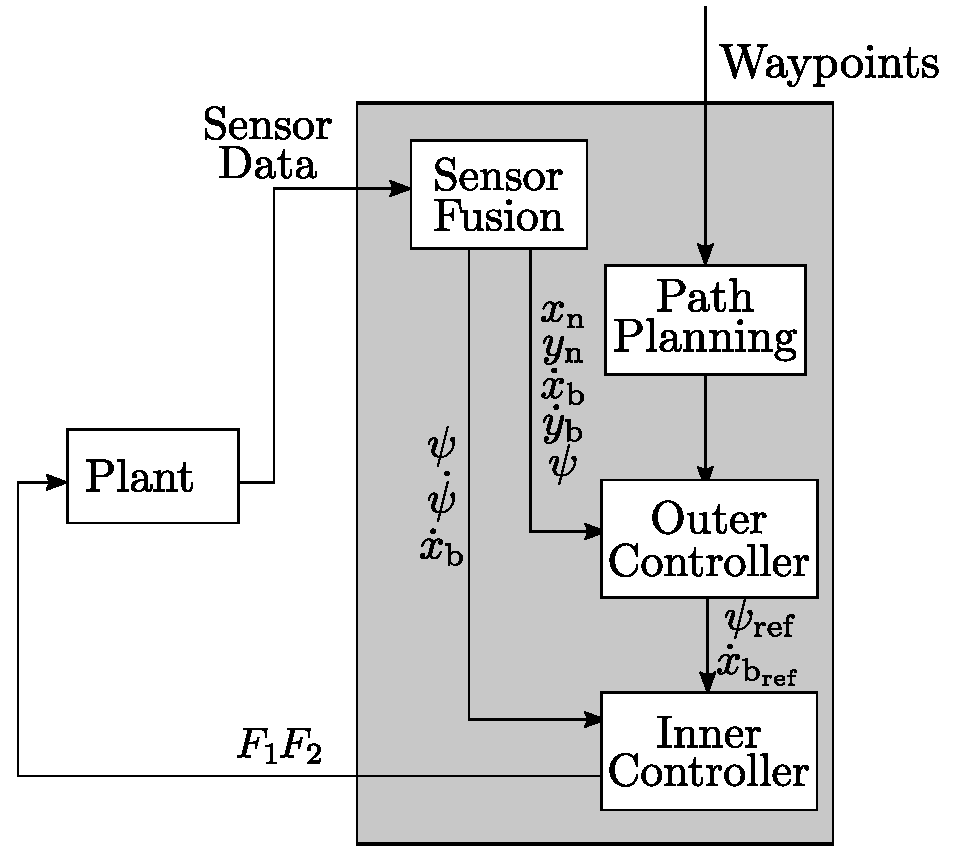
\includegraphics[width=0.3\textwidth]{figures/controllerDiagram2}
    \caption{}
    \label{fig:controllerDiagram}
\end{figure}


The control design consists of two controllers, an inner controller and an outer controller. 

The inner controller uses the references $\dot{x_{bref}}$ and $\dot{\psi_{ref}}$ to regulate $\dot{x_{b}}$ and $\dot{\psi}$ using $F_{1}$ and $F_{2}$. 
Two design approaches will be tested for the inner controller, an $H_{\infty}$ controller and a LQR controller.
The $H_{\infty}$ controller will be designed to be robust towards wind and wave disturbances and towards model errors. 
The LQR controller will be designed to reduce the energy consumption of the vessel, giving the vessel a longer operation period. 

These two approaches will be compared in the end, to see how each compares in the design categories; robustness and energy consumption. 

The outer controller is responsible for maintaining following a path in the inertial frame. 
It receives a set of waypoints from the path planner, which when interpolated represents a desired path for the boat to follow. 
By comparing the measured position of the vessel it is able to compute a heading needed in the inertial frame, which is needed to follow that path.
This is obtained by adjusting the reference of the inner controller. 
%%%%%Sensor Fusion%%%%%%
The sensor fusion is implemented to improve the accuracy of the measurements. 
The sensor fusion ustilizes a kalmann filter to reduce measurement noise from the sensors, by comparing the measurements to a model of the vessel. 

